\chapter{LASER GUIDANCE SYSTEM DESIGN}

\section{Laser Guidance System Overview}
Driving on the farm field faces unpredictable ground conditions all the time, such as rocks, mounds, slides, or rabbit or rat holes. It is impossible for tractors to drive through every thing without deviating from the planned track. However, it is possible to have the attachments of the tractors always stay on the planned track. In order to do so, a physical buffer is designed to be installed on the tractor attachment, and the frame of all the tools on the attachment should connect to the buffer so that they move along with the buffer. Therefore, this buffer is able to keep the field tools independent from the tractor and always on the planned trajectory.
\begin{figure}[ht!]
\begin{center}
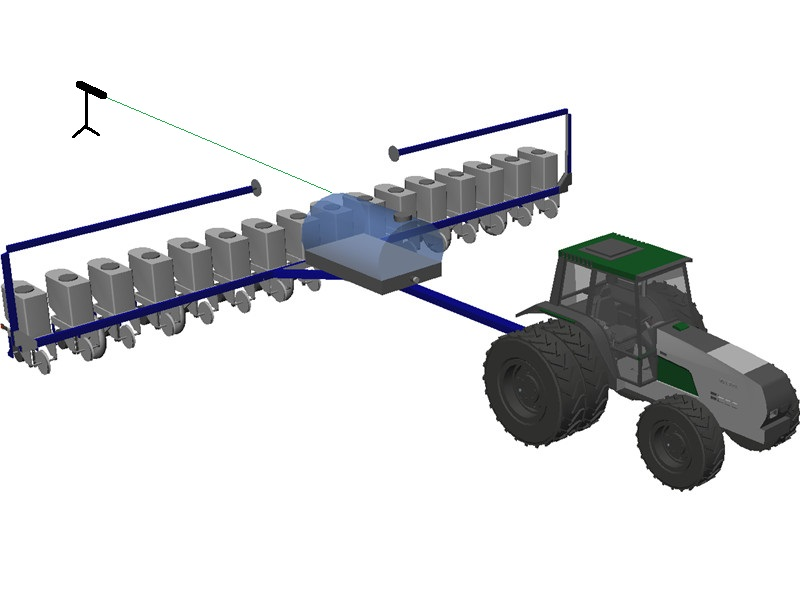
\includegraphics[scale = 0.6]{pics/tractor.jpg}
\caption{Laser guide}
\end{center}
\end{figure}

According to the related researches, vision guidance has been chosen to use as the guidance system for the buffer, because a camera is a low-cost device. In this paper, an additional laser pointer is used as a stable reference. The laser pointer is placed at the end of rows facing to the back of the tractor to provide the guidance (Figure 4.1), so that the buffer can provide a proper compensation to deviation by observing the laser beam. 

In addition, two LEDs can be installed on both the left and right side of the dashboard of the tractor. The LEDs tell the driver to turn the steering wheel left or right to counter the deviation. 
%It is expected to improve the accuracy dramatically from 10 $cm$ to about 2 $cm$. 

%流程图
%增加论点:在驾驶室加装指示灯,这样可使没有任何导航系统的拖拉机精确移动

\section{Physical Buffer}

%描述buffer程序设计
\begin{figure}[ht!]
\begin{center}
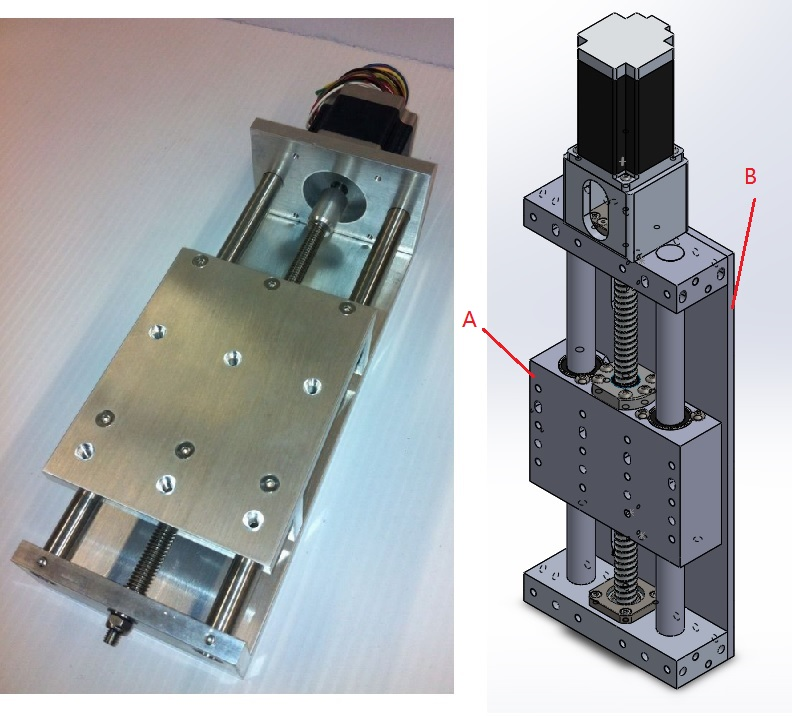
\includegraphics[scale = 0.6]{pics/1D.jpg}
\caption{Linear Sliding Track}
\end{center}
\end{figure}
The design for the physical buffer is to use the linear sliding track (Figure 4.2). There are two sides of the linear sliding track, as the CAD shows in Figure 4.2. Side A connects to the tractor and side B connects to the camera and attachment tools. In addition, considering tractor attachments very heavy, the sliding track must be firm and the stepper motor must be powerful. The physical buffer is installed on the tractor attachments. (Figure 4.3)
\begin{figure}[ht!]
\begin{center}
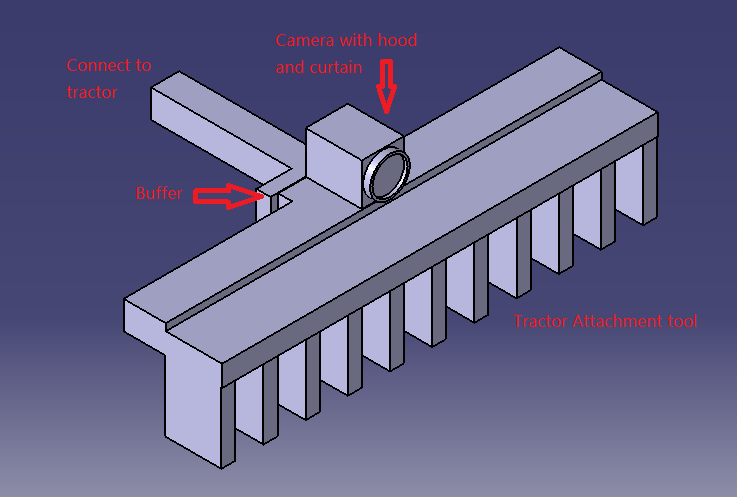
\includegraphics[scale = 0.8]{pics/attachmentwithbuffer.png}
\caption{Tractor with Buffer Installed}
\end{center}
\end{figure} 

The buffer allows the tractor to have some left or right displacement by providing an offset in the opposite direction to the attachment. Therefore, as long as the tractor moves in the right direction and has an accuracy within the offset range of the buffer, the attachment is able to work in a relatively stationary condition. 

\section{Image Processing}
\begin{figure}[ht!]
\begin{center}
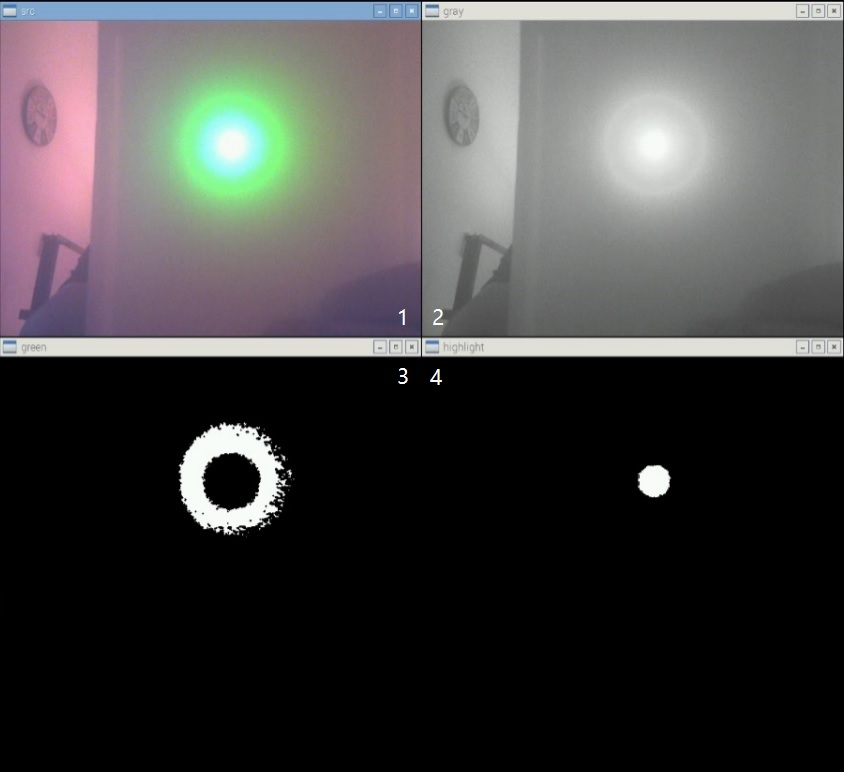
\includegraphics[scale = 0.7]{pics/imaging.jpg}
\caption{Image Processing}
\end{center}
\end{figure}
An image processing algorithm is using to find the position reference from the data gathered by the camera. The algorithm was written in C++ with OpenCV. Several different options were tested.

\subsection{Color Detection}

Color detection was the first method that was implemented and tested. Color detection is straightforward and accurate. Generally, green should be a great color for detection because green has the lowest showing frequency in our daily life, which is why chroma key compositing technology always uses green as the background color. However, green could be everywhere in a crop field, so it is hard to detect the green laser with a green background. To solve this problem, a hood and curtain were attached to the camera to reduce the low intensity lights. Therefore, only the green laser was able to leave a clear green spot on the sight of the a camera. (Figure 4.4 - 1) Although the spot is clear green from human vision, it may not be recognized as green by camera. Under the RGB color space, the "green" spot is always mixed with blue, and sometime red. The color detection is very unreliable, because it could be affected by the surrounding light, thickness of the curtain, and other unknown factors.
\subsection{Improved Color Detection}

According to a related research, the HSV color space has achieved a more accurate performance compared to the original RGB color space. \cite{kaur2013content} To improve the color detection, HSV color space was tested. RGB is well known as red, green, and blue, which are the primary colors of light. Every pixel on a picture contains these three values. Similar to RGB, the three values of HSV are hue, saturation, and value. Unlike the RGB color space where every value has a range from 0 to 255, the values of the HSV color space have different ranges. Hue is the color type, which ranges from 0 to 360 degree. Both saturation and brightness, which is value, range from 0 to 100 percent. The RGB color space is based on the Cartesian coordinate system, but the HSV color space is based on the cylindrical coordinate system. (Figure 4.5)
\begin{figure}[ht!]
\begin{center}
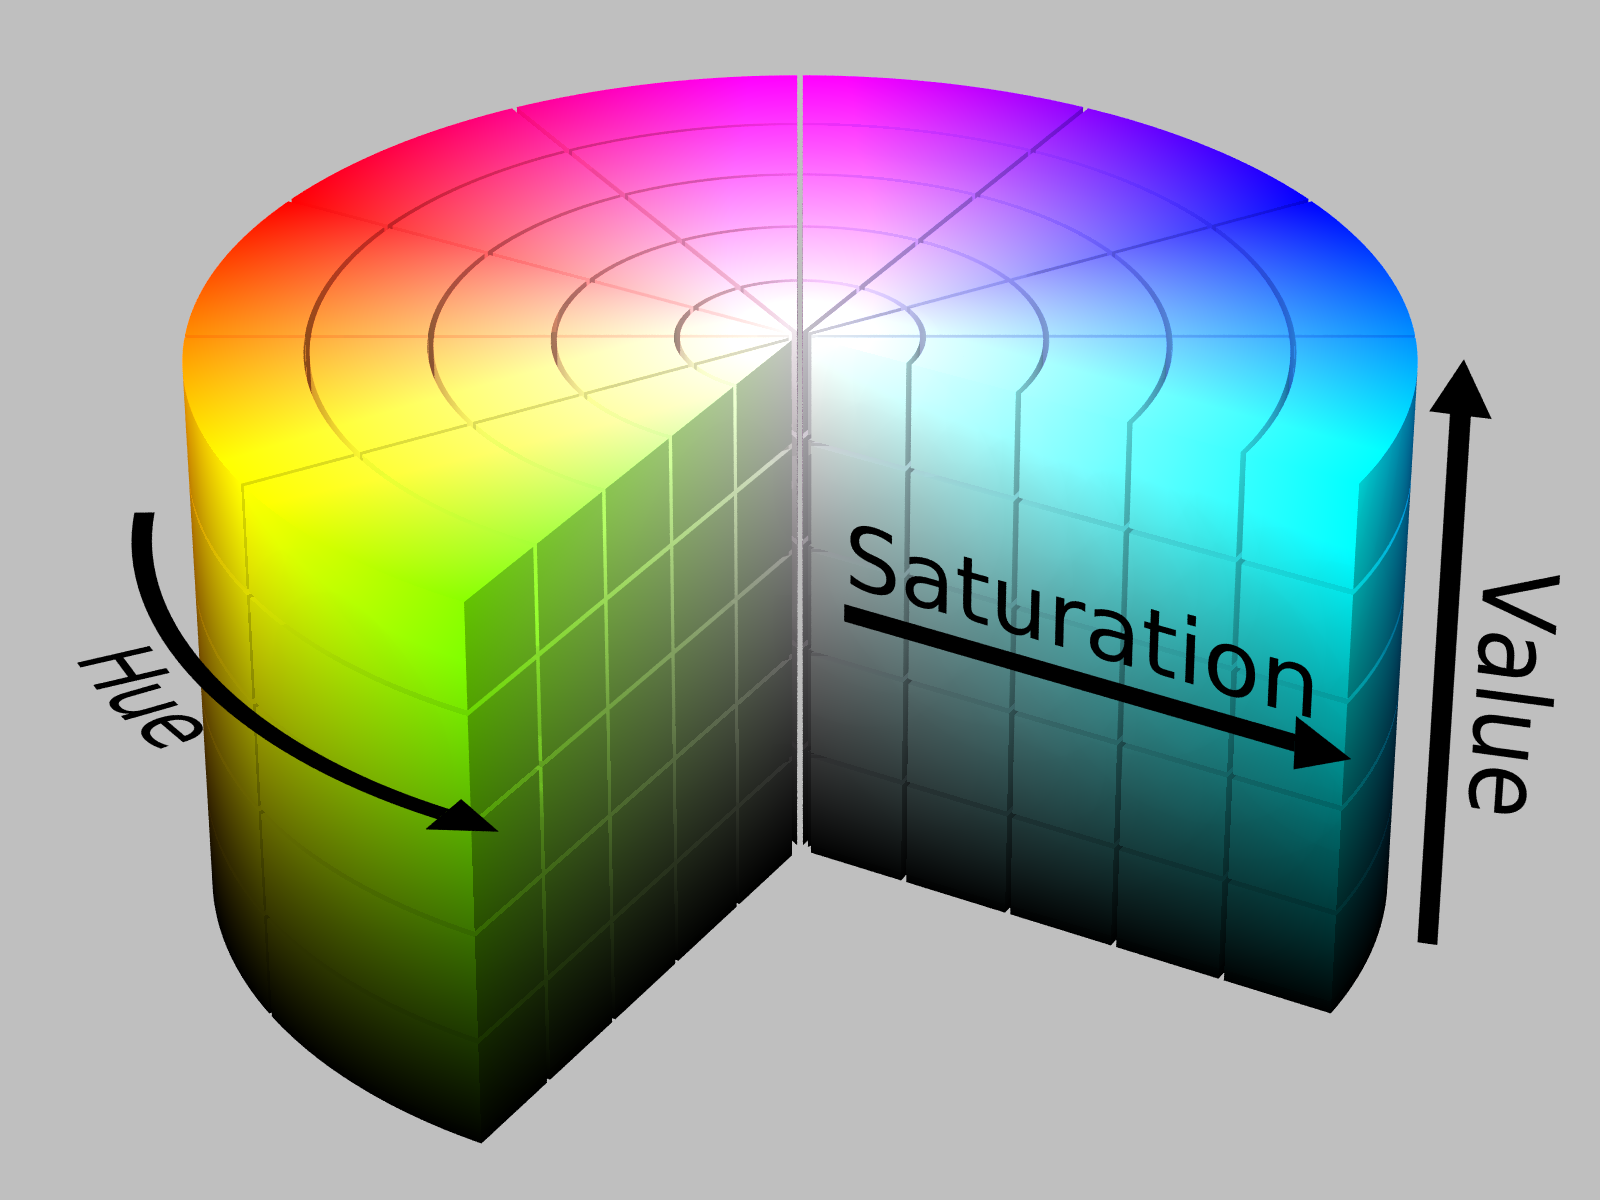
\includegraphics[scale = 0.2]{pics/HSV.png}
\caption{HSV Color Space}
\end{center}
\end{figure}

The conversion formulas are
\begin{equation}
H = cos^{-1}(\frac{\frac{1}{2}[(R-G)+(R-B)]}{\sqrt{(R-G)^{2}+(R-B)(G-B)}})
\end{equation}
\begin{equation}
S = 1-\frac{3}{R+G+B}(min(R,G,B))
\end{equation}
\begin{equation}
V = \frac{1}{3}(R+G+B)
\end{equation}
After the original image transferred from RGB to HSV, a ring-shaped detection was showing on the screen. (Figure 4.4 - 3) The green color detection was stable in the HSV color space, but the ring-shaped detection was unable to provide an accurate coordinate. Unfortunately, there is no way to detect green at the center, because the light intensity at the center is too high for the camera to detect any color.
\subsection{High-Intensity Detection}

For close-distance detection, an additional algorithm was developed. This algorithm only  provides an accurate detection in a close range in order to help color detection. First, the original image was transfered from RGB to GRAY instead of HSV. (Figure 4.4 - 2) Then find the intensity bump was found by masking off all the pixels that were 20 units lower than the maximum intensity. As a result, the detection became a nice point. (Figure 4.4 - 4)

\section{Control Law Design}
This algorithm is defined in the flow chart in Figure 4.6. At the beginning, the camera on the buffer sees the laser spot and sets up the initial position. As the tractor moves, the camera will keep detecting the current position and comparing it with the initial position. Once the left deviation is detected, the buffer will provide the right offset, and the LED on the right will be turned on to tell the driver to turn slightly right. Once the right deviation is detected, the buffer will provide the left offset, and the LED on the left will be turned on to tell the driver to turn slightly left.  In other words, this add-on device will maintain the laser spot in the original position and will notify the driver about detected deviations. 
% Define block styles
\tikzstyle{decision} = [diamond, draw, text width=2.5cm, text badly centered]
\tikzstyle{block} = [rectangle, draw, text width=3cm, text centered, rounded corners, minimum height=1cm]
\tikzstyle{line} = [draw, -latex']
\begin{figure}[ht!]
\begin{center}
\begin{tikzpicture}
\node[block](start) {Start};
\node[block, below = 1 of start] (origin) {Initialize Position};
\node[coordinate, below = 1cm of origin] (cycle) {};
\node[block, left = 2 of cycle](off) {Turn LEDs off};
\node[decision, below = 2 of origin] (L) {Is left deviation detected?};
\node[block, left = 2 of L] (goR) {Provide right offset and turn right LED on};
\node[decision, below = 1 of L] (R) {Is right slide detected?};
\node[block, left = 2 of R] (goL) {Provide deviation offset and turn left LED on};
\node[coordinate, left = 1cm of goR] (left) {};
\node[coordinate, below = 1cm of R] (bottom) {};

\path [line] (start) -- (origin);
\path [line] (origin) -- (L);
\path [line] (L) -- node [anchor = south] {yes} (goR);
\path [line] (goR) -- (left) |- (off);
\path [line] (L) -- node [anchor = east] {no} (R);
\path [line] (R) -- node [anchor = south] {yes} (goL);
\path [line] (goL) -| (left) |- (off);
\path [line] (R) --  node [near start, anchor = east] {no} (bottom) -| (left) |- (off);
\path [line] (off) -- (cycle);
\end{tikzpicture}
\caption{Flow Chart}
\end{center}
\end{figure}